\newpage
\section{51. N皇后}
\label{leetcode:51}

\subsection{题目}

n 皇后问题研究的是如何将 n 个皇后放置在 n×n 的棋盘上,并且使皇后彼此之间不能相互攻击。

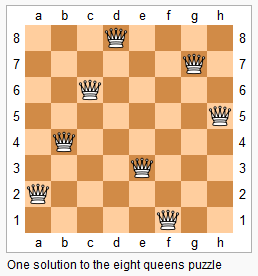
\includegraphics[width=50mm,height=50mm]{images/leetcode/8-queens.png}

上图为 8 皇后问题的一种解法。

给定一个整数 n,返回所有不同的 n 皇后问题的解决方案。

每一种解法包含一个明确的 n 皇后问题的棋子放置方案,
该方案中 \verb|'Q'| 和 \verb|'.'| 分别代表了皇后和空位。

\textbf{示例}:

\begin{verbatim}
输入: 4
输出: [
 [".Q..",  // 解法 1
  "...Q",
  "Q...",
  "..Q."],

 ["..Q.",  // 解法 2
  "Q...",
  "...Q",
  ".Q.."]
]
解释: 4 皇后问题存在两个不同的解法。
\end{verbatim}

\subsection{参考题解}

每一层递归都是进入棋盘中的下一行,然后在每一行中遍历该行的所有列。
判断当前这一行的每个格子是否和上面已经放置好的棋子有冲突。

建立 ``列'',``撇'',``捺'' 3 个 set 来保存已经被占用了位置信息。

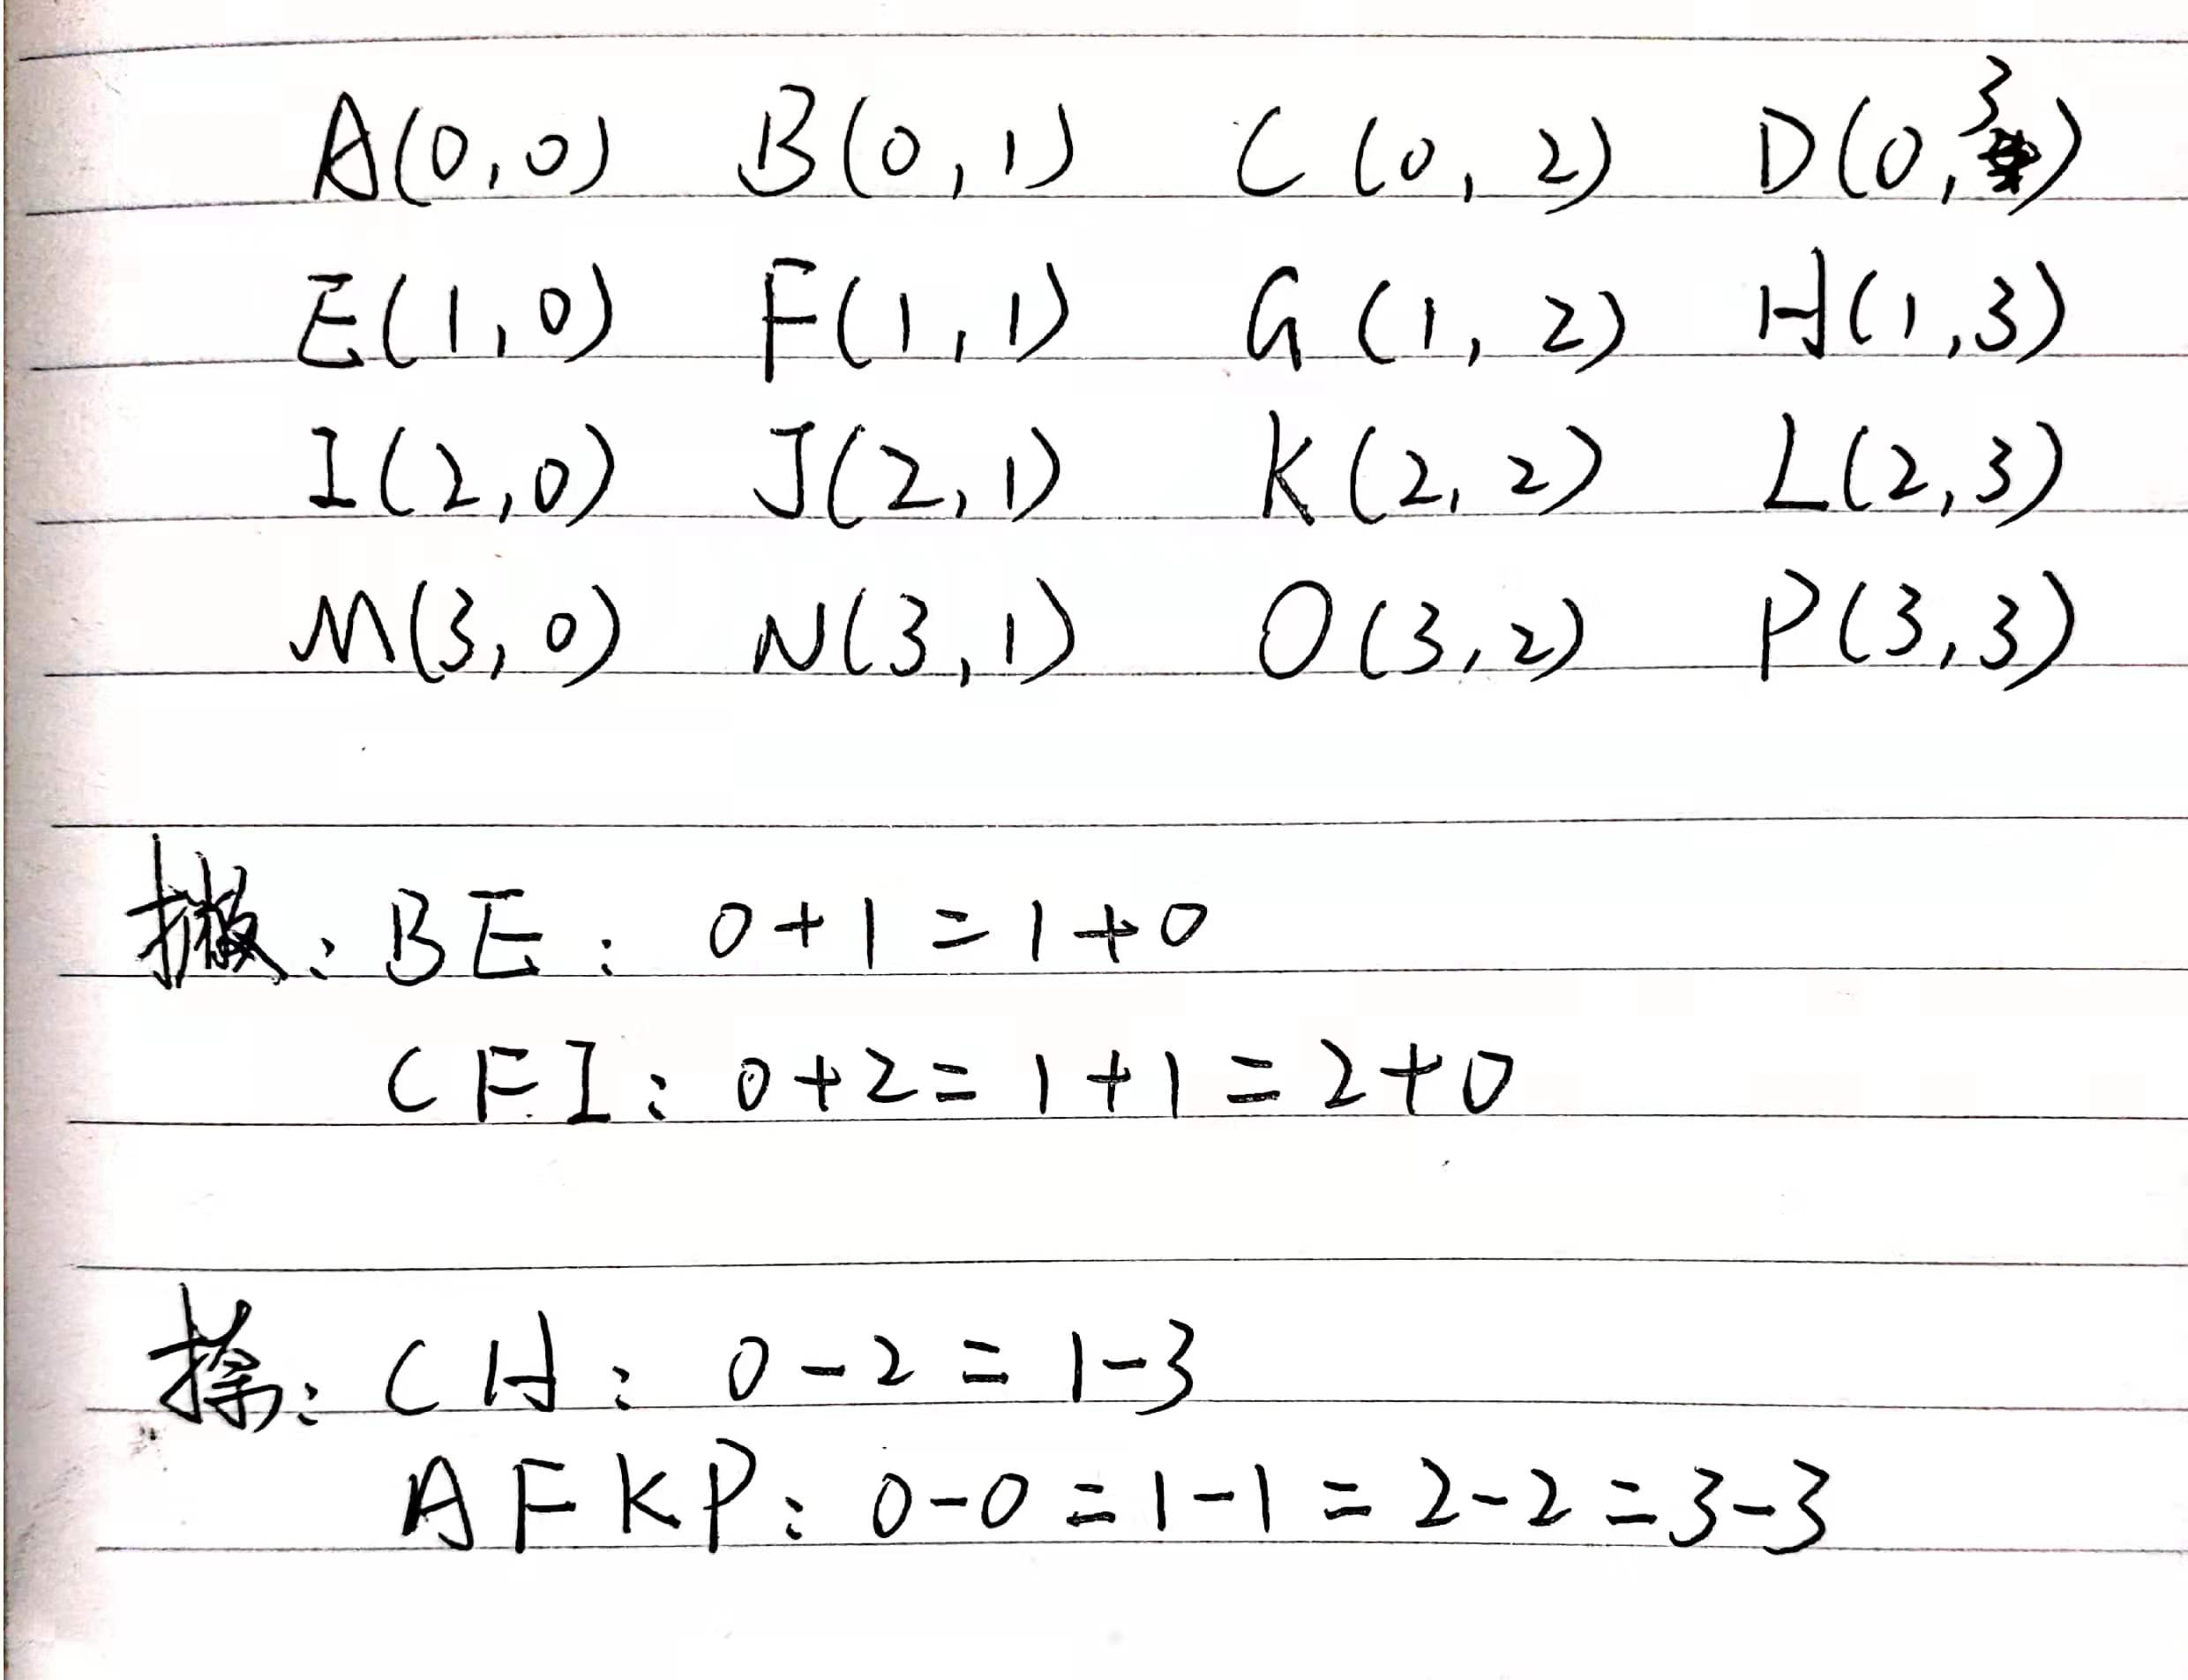
\includegraphics[width=70mm,height=50mm]{images/leetcode/51.jpg}

\begin{verbatim}
/**
 * @param {number} n
 * @return {string[][]}
 */
var solveNQueens = function(n) {
  let result = [];
  dfs(n, 0, [], result, new Set(), new Set(), new Set());

  for (let i = 0; i < result.length; i += 1) {
    for (let j = 0; j < result[i].length; j += 1) {
      const x = result[i][j];
      result[i][j] = '.'.repeat(x) + 'Q' + '.'.repeat(n - x - 1);
    }
  }

  return result;
};

function dfs(n, row, cur, result, cols, pie, na) {
  if (row >= n) {
    result.push(cur.slice());
    return;
  }

  for (let col = 0; col < n; col += 1) {
    if (cols.has(col) ||
      pie.has(row + col) ||
      na.has(row - col)) {
      continue;
    }

    cols.add(col);
    pie.add(row + col);
    na.add(row - col);
    cur.push(col);

    dfs(n, row + 1, cur, result, cols, pie, na);

    cur.pop();
    cols.delete(col);
    pie.delete(row + col);
    na.delete(row - col);
  }
}
\end{verbatim}
